In Section~\ref{sec:language:key_value}, we have presented an algorithm for
replacing a key's value in a BST dictionary. To make the program more
interesting, we consider a sequence of $n$ lookup or replace operations for
different keys in the BST (which may or may not be repeated). A single lookup or
replace has worst-case time complexity $\mathcal{O}(h)$ where $h$ is the height
of the BST, therefore performing $n$ operations takes $\mathcal{O}(h \times n)$
time.

In order to reduce the execution time of the new program, we can cache the
search and replace operations so that repeated operations become faster. Instead
of traversing the entire height of the BST, we look in the cache and send the
operation immediately to the node where the key is located. Without thread
facts, we might have cached the results at the root node, however, this is not a
scalable approach as it would introduce a serious bottleneck.

Figure~\ref{code:threads:btree_lookup_cache} shows the updated BST code with a thread
cache. We just added two more predicates, \code{cache} and
\code{cache-size}, that are facts placed in the thread and represent cached
keys and the total size of the cache, respectively. We also added three new
rules that handle the following cases:

\begin{enumerate}
      \item A key is found and is also in the cache
         (lines~\ref{line:threads:kv_rule1_start}-\ref{line:threads:kv_rule2_end}
         in Fig.~\ref{code:threads:btree_lookup_cache});

      \item A key is found but is not in the cache
         (lines~\ref{line:threads:kv_rule2_start}-\ref{line:threads:kv_rule2_end}
         in Fig.~\ref{code:threads:btree_lookup_cache});

      \item A key is in the cache, therefore a \code{replace} fact is
         derived in the target node
         (lines~\ref{line:threads:kv_rule3_start}-\ref{line:threads:kv_rule3_end}).

\end{enumerate}

Note that it is quite easy to extend the cache mechanism to use an LRU type
approach in order to limit the size of the cache.

\begin{figure}[ht]
\begin{Verbatim}[numbers=left,fontsize=\codesize,commandchars=*\{\}]
type left(node, node).*hfill// Predicate declaration
type right(node, node).
type linear value(node, int Key, string Value).
type linear replace(node, int Key, string Value).
type linear cache(thread, node, int).
type linear cache-size(thread, int).

replace(A, Key, RValue),*hfill*label{line:threads:kv_rule1_start}// Rule 1: key exists and is also in the cache
value(A, Key, Value),
*underline{cache(T, A, Key)}
   -o value(A, Key, RValue).
      *underline{cache(T, A, Key)}.*label{line:threads:kv_rule1_end}

replace(A, Key, RValue),*label{line:threads:kv_rule2_start}*hfill// Rule 2: key exists and is not in the cache
value(A, Key, Value),
*underline{cache-size(T, Total)}
   -o value(A, Key, RValue),
      *underline{cache-size(T, Total + 1)},
      *underline{cache(T, A, Key)}.*label{line:threads:kv_rule2_end}

replace(A, RKey, RValue),*label{line:threads:kv_rule3_start}*hfill// Rule 3: cached by the thread
*underline{cache(T, TargetNode, RKey)}
   -o replace(TargetNode, RKey, RValue),
      *underline{cache(T, TargetNode, RKey)}.*label{line:threads:kv_rule3_end}

replace(A, RKey, RValue),*hfill// Rule 4: go left
value(A, Key, Value),
!left(A, B),
RKey < Key
   -o value(A, Key, Value),
      replace(B, RKey, RValue).

replace(A, RKey, RValue),*hfill// Rule 5: go right
value(A, Key, Value),
!right(A, B),
RKey > Key
   -o value(A, Key, Value),
      replace(B, RKey, RValue).
\end{Verbatim}
\caption{LM program for performing lookups in a BST extended to use a thread cache.}
\label{code:threads:btree_lookup_cache}
\end{figure}

\begin{table}[ht]
   \begin{center}
      \begin{tabular}{c | c || c c | c c | c c} \hline
	 \multirow{2}{*}{\textbf{Dataset}} & \multirow{2}{*}{\textbf{Threads}} & \multicolumn{2}{c|}{\textbf{\# Derived}} & \multicolumn{2}{c|}{\textbf{\# Deleted}} & \multicolumn{2}{c}{\textbf{\# Final}}\\
	 & & Regular & Cached & Regular & Cached & Regular & Cached\\ \hline \hline
\multirow{7}{*}{19 levels}  & 1 &  45.6M & 10.5M &  42.4M & 7.4M &  3.1M & 3.2M \\
 & 2 &  45.6M & 13.7M &  42.4M & 10.5M &  3.1M & 3.2M \\
 & 4 &  45.6M & 16.1M &  42.4M & 13.3M &  3.1M & 3.2M \\
 & 8 &  45.6M & 17.5M &  42.4M & 14.3M &  3.1M & 3.2M \\
 & 16 &  45.6M & 23.6M &  42.4M & 20.4M &  3.1M & 3.2M \\
 & 24 &  45.6M & 29.6M &  42.4M & 26.4M &  3.1M & 3.2M \\
 & 32 &  45.6M & 31.9M &  42.4M & 28.7M &  3.1M & 3.2M \\
	\hline
\multirow{7}{*}{21 levels}  & 1 &  126.5M & 30.6M &  116.9M & 21.8M &  9.6M & 9.8M \\
 & 2 &  126.5M & 35.7M &  116.9M & 26.1M &  9.6M & 9.8M \\
 & 4 &  126.5M & 43.1M &  116.9M & 33.4M &  9.6M & 9.8M \\
 & 8 &  126.5M & 52.1M &  116.9M & 42.4M &  9.6M & 9.8M \\
 & 16 &  126.5M & 64.5M &  116.9M & 54.7M &  9.6M & 9.8M \\
 & 24 &  126.5M & 73.5M &  116.9M & 63.6M &  9.6M & 9.8M \\
 & 32 &  126.5M & 83.7M &  116.9M & 73.8M &  9.6M & 9.8M \\
	\hline
\end{tabular}

   \end{center}

   \caption{Fact statistics for the \textbf{Regular} version and the
   \textbf{Cached} version.}
   \label{results:threads:key_value}
\end{table}

\begin{figure}[]
        \centering
        \begin{subfigure}[b]{\plotsize\textwidth}
           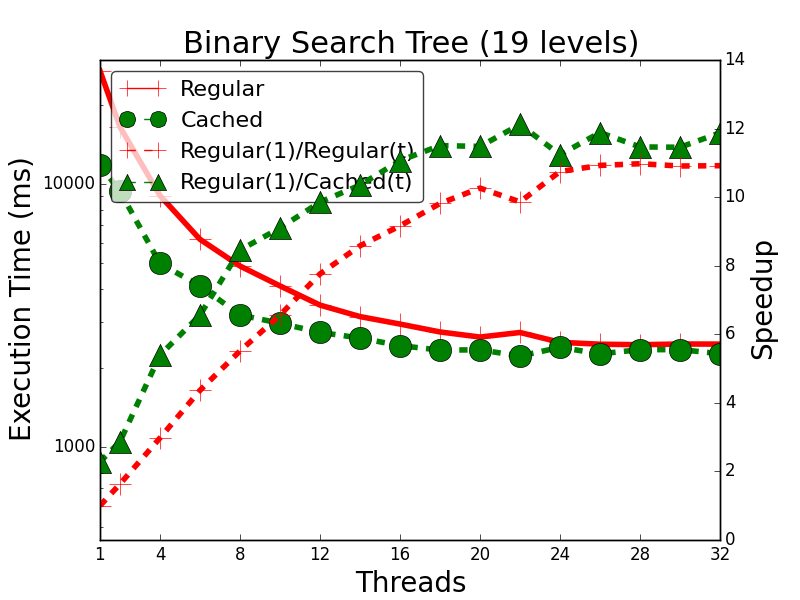
\includegraphics[width=\textwidth]{experiments/threads/cmp-key-value-19-ten.png}
           \label{fig:threads:key_value_19}
        \end{subfigure}
        ~
        \begin{subfigure}[b]{\plotsize\textwidth}
           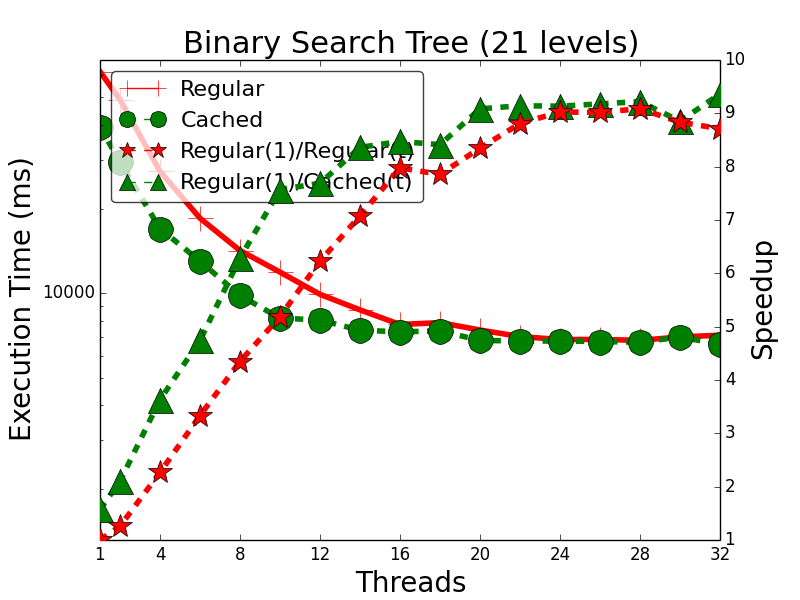
\includegraphics[width=\textwidth]{experiments/threads/cmp-key-value-21-ten.png}
           \label{fig:threads:key_value_21}
        \end{subfigure} \\

        \caption{Scalability for the Binary Search Tree program when using
        thread based facts.}

        \label{fig:threads:results_key_value}
\end{figure}

\clearpage
